 


% Copyright 2004 by Till Tantau <tantau@users.sourceforge.net>.
%
% In principle, this file can be redistributed and/or modified under
% the terms of the GNU Public License, version 2.
%
% However, this file is supposed to be a template to be modified
% for your own needs. For this reason, if you use this file as a
% template and not specifically distribute it as part of a another
% package/program, I grant the extra permission to freely copy and
% modify this file as you see fit and even to delete this copyright
% notice. 

\documentclass{beamer}

% There are many different themes available for Beamer. A comprehensive
% list with examples is given here:
% http://deic.uab.es/~iblanes/beamer_gallery/index_by_theme.html
% You can uncomment the themes below if you would like to use a different
% one:
%\usetheme{AnnArbor}
%\usetheme{Antibes}
%\usetheme{Bergen}
%\usetheme{Berkeley}
%\usetheme{Berlin}
%\usetheme{Boadilla}
%\usetheme{boxes}
%\usetheme{CambridgeUS}
%\usetheme{Copenhagen}
%\usetheme{Darmstadt}
%\usetheme{default}
%\usetheme{Frankfurt}
%\usetheme{Goettingen}
%\usetheme{Hannover}
%\usetheme{Ilmenau}
%\usetheme{JuanLesPins}
%\usetheme{Luebeck}
\usetheme{Madrid}
%\usetheme{Malmoe}
%\usetheme{Marburg}
%\usetheme{Montpellier}
%\usetheme{PaloAlto}
%\usetheme{Pittsburgh}
%\usetheme{Rochester}
%\usetheme{Singapore}
%\usetheme{Szeged}
%\usetheme{Warsaw}

%==========Packages================
\usepackage[utf8]{inputenc}
    \usepackage[T1]{fontenc} 
    \usepackage[francais]{babel}
    \usepackage{amsmath}
    \usepackage{amssymb}
    \usepackage{graphicx}
    \usepackage{color}
    \usepackage{hyperref}
    \usepackage[left=2cm,right=2cm,top=2cm,bottom=2cm]{geometry}
    \usepackage{mathrsfs}
    \usepackage{verbatim}
%========================================


    \title{Application de chiffrement homomorphe à l'apprentissage automatique}

% A subtitle is optional and this may be deleted
    \subtitle{Optional Subtitle}
    \author{BENISSA Sami \\
      Université Paris 8\\
    Master BLA}
%\author{F.~Author\inst{1} \and S.~Another\inst{2}}
% - Give the names in the same order as the appear in the paper.
% - Use the \inst{?} command only if the authors have different
%   affiliation.

\institute[Jolibrain, Toulouse, France] % (optional, but mostly needed)
%{
 % \inst{1}%
  %Master BLABLA\\
  %Département BLABLA\\
  %Université Paris 8
  %\and
  %\inst{2}%
  %Department of Theoretical Philosophy\\
  %niversity of Elsewhere}
% - Use the \inst command only if there are several affiliations.
% - Keep it simple, no one is interested in your street address.

\date{Jeudi 28 Septembre, 2017}
% - Either use conference name or its abbreviation.
% - Not really informative to the audience, more for people (including
%   yourself) who are reading the slides online

%\subject{Theoretical Computer Science}
% This is only inserted into the PDF information catalog. Can be left
% out. 

% If you have a file called "university-logo-filename.xxx", where xxx
% is a graphic format that can be processed by latex or pdflatex,
% resp., then you can add a logo as follows:

% \pgfdeclareimage[height=0.5cm]{university-logo}{university-logo-filename}
% \logo{\pgfuseimage{university-logo}}

% Delete this, if you do not want the table of contents to pop up at
% the beginning of each subsection:

\AtBeginSection[]
{
  \begin{frame}<beamer>{Déroulement}
    \tableofcontents[currentsection]
  \end{frame}
}

\AtBeginSubsection[]
{
  \begin{frame}<beamer>{Déroulement}
    \tableofcontents[currentsection,currentsubsection]
  \end{frame}
}

% Let's get started
\begin{document}

\begin{frame}
  \titlepage
\end{frame}

\begin{frame}{Déroulement}
  \tableofcontents
  % You might wish to add the option [pausesections]
\end{frame}

% Section and subsections will appear in the presentation overview
% and table of contents.
\section{Présentation de l'entreprise}

%\subsection{First Subsection}

%////////////SLIDE1\\\\\\\\\\\\\\\\\\
\begin{frame}{Présentation de l'entreprise}{Jolibrain, Toulouse}
\begin{itemize}
  \item {
    Vétérans de l'Intelligence artificielle et du Web\\
    +Expert
    \pause % The slide will pause after showing the first item
  }
  \item {   
    Open Source
    \pause
  }
    \item {   
      Machine Learning, Deep Learning, Reinforcement Learning, Stochastic Optimization, Search Enginesengin de recherche, system P2P \\
      etc...
    \pause
    }
\end{itemize}
\end{frame}
%\\\\\\\\\\\\\\\\\\\////////////////////

%/////////////////NEW SLIDE\\\\\\\\\\\\\\\\\\
  

\section{Introduction}


%//////////////////////NEW SLIDE\\\\\\\\\\\\\\\\\
%\subsection{Contexte : Big data et Intelligence Artificielle}

\begin{frame}{Introduction}
\begin{block}{Contexte}
Big data et Intelligence Artificielle
\end{block}

%\subsection{Problématique : Ethique et confidentialité}

\begin{block}{Problématique}
Ethique et confidentialité.
\end{block}

%\subsection{Objectifs du stage}

\begin{block}{Objectif du stage}
Concevoir une application d'apprentissage automatique a partir des données chiffrées en utilisant un schéma de chiffrement homomorphe.
\end{block}
\end{frame}

%
%%%
\section{Etat de l'art}
  
%%%  

%////////////////////////NEW SLIDE\\\\\\\\\\\\\\\\\\\\

  \begin{frame}{Etat de l'art}

    \begin{itemize}
  \item {
    Cryptographie
  }
  \item {
    ML
  }
    \item {
    Cryptographie + ML
  }
  \end{itemize}
\end{frame}

  \subsection{Cryptographie}
  
  %////////////////////////NEW SLIDE\\\\\\\\\\\\\\\\\\\\
  %Chiffrement partiellement homomorphe définition
  \begin{frame}{Cryptographie}

    \begin{itemize}
    \item<1-> {
      Chiffrement partiellement homomorphe : Définition :\\
      \uncover<2->{Si on considère $C$ un cryptosystème,} \\

     \begin{itemize}[label={}]
           \item[]<3-> {
             $(x_1, x_2, ............, x_n)$ , l'ensemble de messages clairs, 
           }
           \item[]<4-> {  
             $(c_1, c_2, ..............., c_n)$ , l'ensemble des messages chiffrés
           }
           \item[]<5-> {
        et $ F$ une fonction de chiffrement telle que:\\
        $$F(x_n) = c_n$$
           }\\
     \end{itemize}

             \uncover<6-> {On dit que $C$ est homomorphique par rapport a l'addition si : \\
               $$F(x_1) + F(x_2) = F(x_1 + x_2).$$
                           }\\
      \uncover<7-> {On dit que $C$ est homomorphique par rapport a la multiplication si : \\
 $$F(x_1) * F(x_2) = F(x_1 * x_2).$$}
          }   
    
  \end{itemize}
\end{frame}

  %\\\\\\\\\\\\\\\\\\\\\\\\\\///////////////////////


   %////////////////////////NEW SLIDE\\\\\\\\\\\\\\\\\\\\
  %RSA, description
  \begin{frame}{Cryptographie}

    \begin{itemize}
    \item<1-> {
      RSA :
              }
    \end{itemize}

  \end{frame}


  
 %\\\\\\\\\\\\\\\\\\\\\\\\\\///////////////////////


   %////////////////////////NEW SLIDE\\\\\\\\\\\\\\\\\\\\
  %Paillier, description
  \begin{frame}{Cryptographie}

    \begin{itemize}
    \item<1-> {
      Paillier :
              }
    \end{itemize}

  \end{frame}


  %//////////////NEW SLIDE\\\\\\\\\\\\\\\\\\\\\
  %Crypto completement homomorphe
  \begin{frame}{Cryptographie}

    \begin{itemize}
    \item<1-> {
      Chiffrement complètement homomorphe\\
      \uncover<2->{Un cryptosystème est dit homomorphe si une opération algébrique effectuée sur les chiffrés équivaut à une opération algébrique sur les clairs. En particulier, si le cryptosystème est stable pour un nombre arbitraire d'additions et de multiplications, il est dit complètement homomorphe.} \\
              }
    
  \end{itemize}
  \end{frame}
  %\\\\\\\\\\\\\\\\\\\·/////////////////////
  

  %//////////////NEW SLIDE\\\\\\\\\\\\\\\\\\\\\
  %Réseaux Euclidiens
  \begin{frame}{Cryptographie}

    \begin{itemize}
    \item<1-> {
      Réseaux Euclidiens : \\
      \uncover<2->{ Un réseau euclidien $L$ est un sous-groupe discret additif de $R^n$.\\
      }
      \uncover<3->{ une base $b= (b_1,b_2,...........,b_n)$ de $L$ dans $R^n$ est un ensemble de $n$ vecteurs linéairement indépendants.\\
        Les combinaisons linéaires entières des vecteurs de cette base forment $L$.
$$L = \{x\in R^n, tq\quad x = \sum_{i=1}^{n} x_ib_i,\quad x_i\in Z\}$$
      }
      \uncover<4->{\begin{figure}[h!]\begin{center}
                   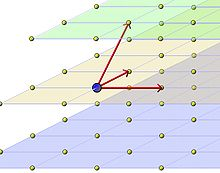
\includegraphics[width=3cm]{reseau.jpg}
                   \caption{Réseau euclidien de dimension 3 .}
                   \end{center}
                   \end{figure}
      }
      }
    
  \end{itemize}
  \end{frame}
  %\\\\\\\\\\\\\\\\\\\·/////////////////////

   %//////////////NEW SLIDE\\\\\\\\\\\\\\\\\\\\\
  %SVP et CVP
  \begin{frame}{Cryptographie}

    \begin{itemize}
    \item<1-> {
      \textbf{Shortest Vector Problem (SVP):}\\
      \uncover<2->{Etant donné une base $B$ d’un sous réseau $L$ de $Z^n$, trouver un vecteur non nul de $L$ le plus court possible pour la norme euclidienne.}\\
      \uncover<3->{
      \begin{figure}[h!]\begin{center}
          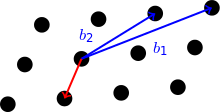
\includegraphics[width=3cm]{svp.png}
          \caption{En bleu la base donnée du réseau, en rouge le vecteur le plus court.}
    %\label{fig:svp}
        \end{center}
      \end{figure}
      }
    }
    \item<4->{
      \textbf{Closest Vector Problem (CVP):}\\
      \uncover<5->{Etant donné une base $B$ d’un réseau $L$ de $Z^n$ et un vecteur $v \in Q^n$ , trouver le vecteur de $L$ le plus proche de $v$ pour la norme euclidienne.}\\
      \uncover<6->{
        \begin{figure}[h!]\begin{center}
            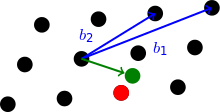
\includegraphics[width=3cm]{cvp.png}
            \caption{En bleu la base donnée du réseau, en vert le vecteur donné,en rouge le vecteur le plus proche du vecteur vert appartenant au réseau.}
            \label{fig:cvp}
          \end{center}
        \end{figure}
      }
    }
    \end{itemize}
  \end{frame}

  %//////////////NEW SLIDE\\\\\\\\\\\\\\\\\\\\\
  %Gentry
  \begin{frame}{Cryptographie}

    \begin{itemize}
    \item<1-> {
      \textbf{Cryptosystème de Gentry}\
      \uncover<2->{A toi de remplir} \\
              }
  \end{itemize}
  \end{frame}
  %\\\\\\\\\\\\\\\\\\\·/////////////////////
  
%//////////////NEW SLIDE\\\\\\\\\\\\\\\\\\\\\
  %BGV
  \begin{frame}{Cryptographie}

    \begin{itemize}
    \item<1-> {
      \textbf{Le cryptosystème Brakerski-Gentry-Vaikunthanathan (BGV)}\
      \uncover<2->{A toi de remplir} \\
              }
  \end{itemize}
  \end{frame}
  %\\\\\\\\\\\\\\\\\\\·/////////////////////


  \subsection{Apprentissage automatique}
 
%//////////////NEW SLIDE\\\\\\\\\\\\\\\\\\\\\
  %ML
  \begin{frame}{Apprentissage automatique}

    \begin{itemize}
    \item<1-> {
      \textbf{Apprentissage automatique \textit{Machine Learning - ML}}\\
      \uncover<2->{A toi de remplir} \\
              }
  \end{itemize}
  \end{frame}
  %\\\\\\\\\\\\\\\\\\\·/////////////////////

  \subsection{Cryptographie + ML}

  %//////////////NEW SLIDE\\\\\\\\\\\\\\\\\\\\\
  %BGV
  \begin{frame}{Apprentissage automatique}

    \begin{itemize}
    \item<1-> {
      \textbf{Crypto + ML}\\
      \uncover<2->{Pour certaines données sensibles, il n'est pas pensable d'effectuer des calculs sur le cloud. Pour pallier à ce problème de confidentialité et de sécurité, il est nécessaire de combiner ML et crypto} \\
      \uncover<3->{
        \begin{figure}[h!]\begin{center}
            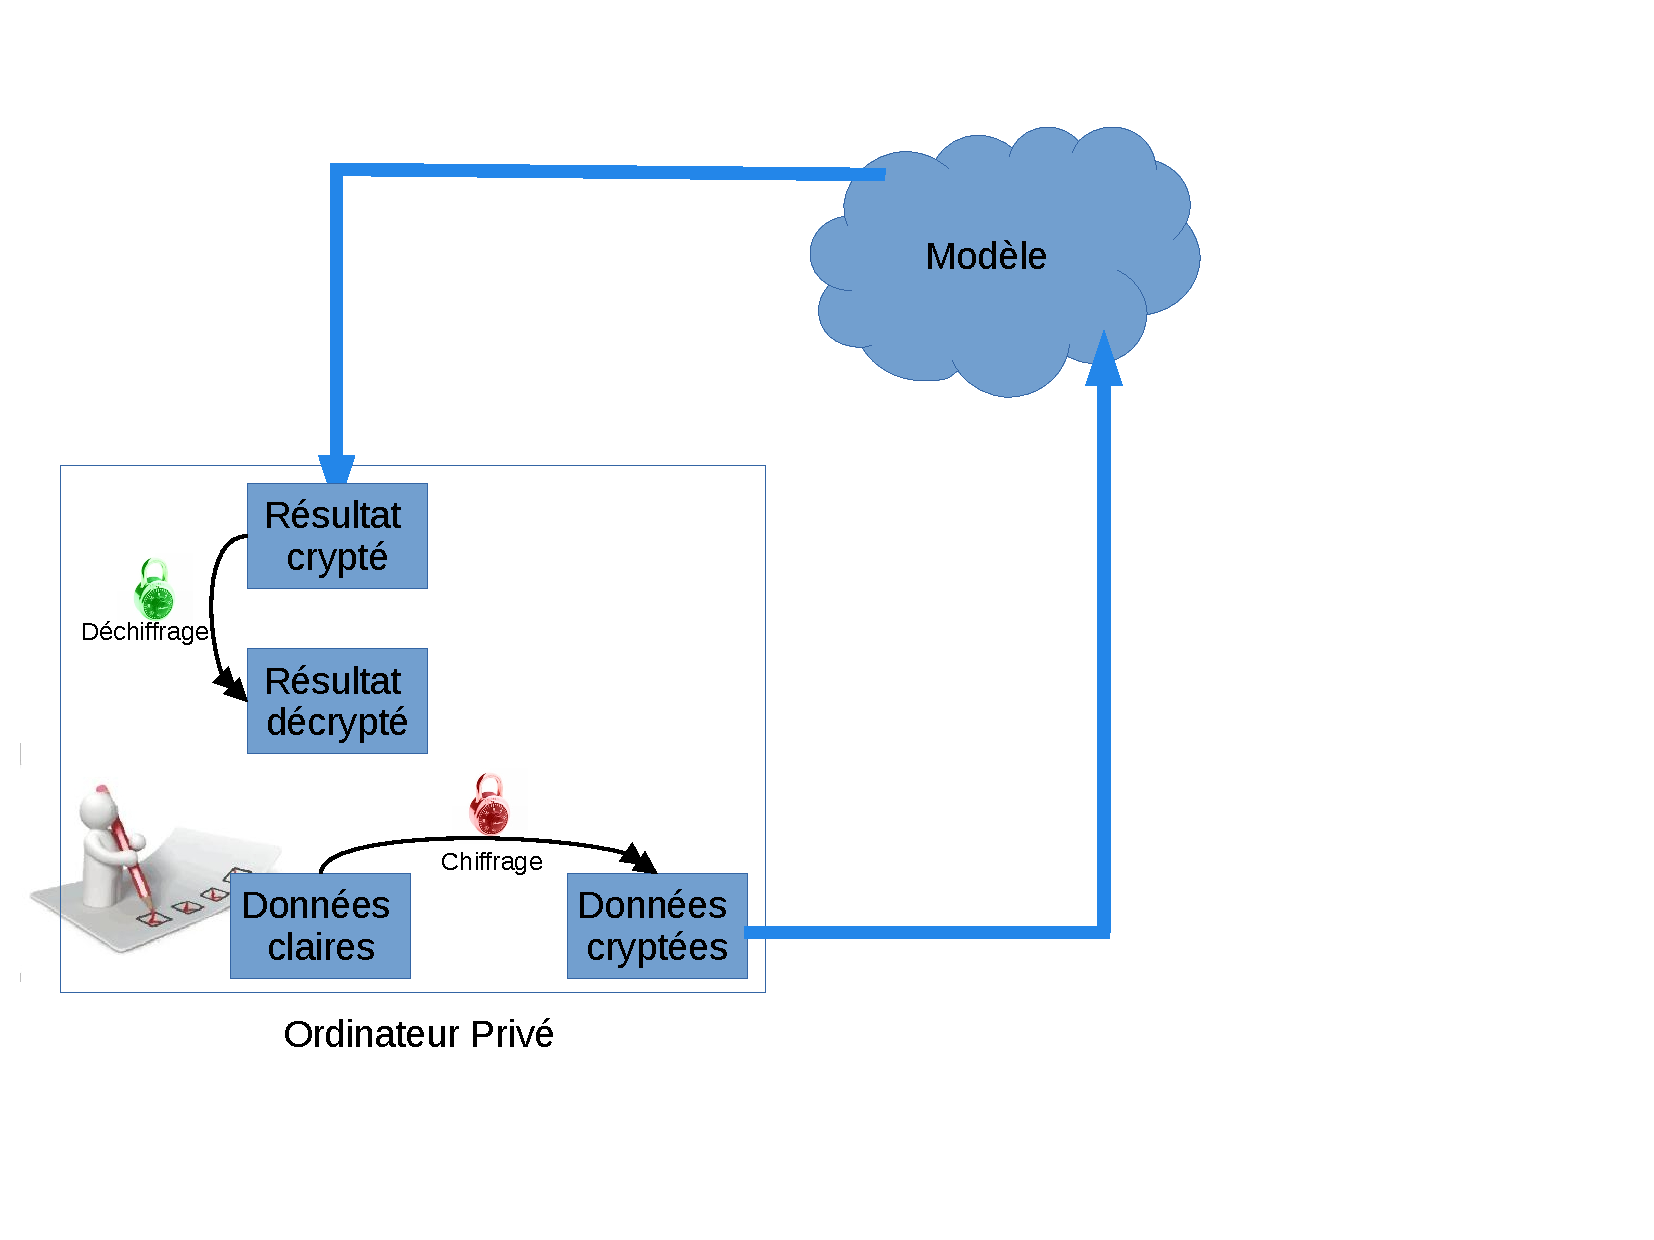
\includegraphics[width=5cm]{SchemaM1.pdf}
          \end{center}
        \end{figure}
      }
              }
  \end{itemize}
  \end{frame}
  %\\\\\\\\\\\\\\\\\\\·/////////////////////
  
%//////////////COMMENTAIRE\\\\\\\\\\\\\\\\\\\
\begin{comment}
\begin{frame}{Blocks}
\begin{block}{Block Title}
You can also highlight sections of your presentation in a block, with it's own title
\end{block}
\begin{theorem}
There are separate environments for theorems, examples, definitions and proofs.
\end{theorem}
\begin{example}
Here is an example of an example block.
\end{example}
\end{frame}

%\\\\\\\\\\\\\\\\\\\\//////////////////////

\begin{frame}
  \begin{itemize}
  \item {
    My first point.
  }
  \item {
    My second point.
  }
  \end{itemize}
\end{frame}

\subsection{Second Subsection}

% You can reveal the parts of a slide one at a time
% with the \pause command:
\begin{frame}{Second Slide Title}
  \begin{itemize}
  \item {
    First item.
    \pause % The slide will pause after showing the first item
  }
  \item {   
    Second item.
  }
  % You can also specify when the content should appear
  % by using <n->:
  \item<3-> {
    Third item.
  }
  \item<4-> {
    Fourth item.
  }
  % or you can use the \uncover command to reveal general
  % content (not just \items):
  \item<5-> {
    Fifth item. \uncover<6->{Extra text in the fifth item.}
  }
  \end{itemize}
\end{frame}

% Placing a * after \section means it will not show in the
% outline or table of contents.
\section*{Summary}

\begin{frame}{Summary}
  \begin{itemize}
  \item
    The \alert{first main message} of your talk in one or two lines.
  \item
    The \alert{second main message} of your talk in one or two lines.
  \item
    Perhaps a \alert{third message}, but not more than that.
  \end{itemize}
  
  \begin{itemize}
  \item
    Outlook
    \begin{itemize}
    \item
      Something you haven't solved.
    \item
      Something else you haven't solved.
    \end{itemize}
  \end{itemize}
\end{frame}



% All of the following is optional and typically not needed. 
\appendix
\section<presentation>*{\appendixname}
\subsection<presentation>*{For Further Reading}

\begin{frame}[allowframebreaks]
  \frametitle<presentation>{For Further Reading}
    
  \begin{thebibliography}{10}
    
  \beamertemplatebookbibitems
  % Start with overview books.

  \bibitem{Author1990}
    A.~Author.
    \newblock {\em Handbook of Everything}.
    \newblock Some Press, 1990.
 
    
  \beamertemplatearticlebibitems
  % Followed by interesting articles. Keep the list short. 

  \bibitem{Someone2000}
    S.~Someone.
    \newblock On this and that.
    \newblock {\em Journal of This and That}, 2(1):50--100,
    2000.
  \end{thebibliography}
\end{frame}

\end{comment}
%%%%%%%%%%%%%%%%%%%fin du comment
\end{document}


